\documentclass[11pt, a4paper]{scrreprt}  % Koma-Script Style Paket für Reports - nach Markus Kohm
\usepackage[left=3cm, right=3cm, top=3cm]{geometry}  % 'geometry'-Paket erlaubt u.a. die Festlegung der Seitenränder
\usepackage[utf8]{inputenc} % Kodierung der Non-ASCII-Zeichen
\usepackage[OT1]{fontenc}
\renewcommand*\familydefault{\sfdefault} % Schriftart sans serif

\usepackage[german,ngerman]{babel}  % neue deutsche Rechtschreibung
\usepackage{tabto}  % Tabulatoren
\usepackage{lipsum} % lorem ipsum- Leertexte
\usepackage{graphicx}

\newtheorem{question}{Frage}

\begin{document}
\thispagestyle{empty}
\pdfbookmark[0]{Titelblatt}{title}

\begin{titlepage}

%\vspace*{\stretch{1}}

\begin{center}

{\huge Fernuniversität Hagen} \\ [1,0cm]

{\Large Modul 63458 - Fachpraktikum \\ [0,3 cm]
Natural Language Processing, Information Extraction und Retrieval \\ [0,3 cm]
WiSe 2022/23} \\ [3cm]

{\huge Praktikumsbericht}

\vspace{8ex}

{\huge\bfseries
Automatische Erstellung \\[0,5cm]
einer Wissensrepräsentation \\[0,5cm]
aus einem medizinischen Text \\[0,5cm]
}

\vspace{8ex}

{\large eingereicht von}

\vspace{4ex}

{\Large Anne Koch, Clara Jansen, Dietrich Tönnies}
 
\end{center}

\vspace{6ex}

{\Large \hspace{2,4cm} Betreuer: \tabto{5,5cm} Prof. Dr. Hemmje
\vspace{0,2cm}
\tabto{5,5cm}  Dr. Christian Nawroth
\vspace{0,5cm}
\tabto{5,5cm} Stephanie Heidepriem, M.Sc.}

\vfill

\begin{center}
{\large Hagen, \today}
\end{center}

\end{titlepage}


\tableofcontents
\automark[section]{chapter}
\renewcommand{\chaptermark}[1]{\markboth{\spacedlowsmallcaps{#1}}{\spacedlowsmallcaps{#1}}}
\renewcommand{\sectionmark}[1]{\markright{\thesection\enspace\spacedlowsmallcaps{#1}}}
\refstepcounter{dummy}
\setcounter{secnumdepth}{2} 

\chapter{Einleitung}

Diese Praktikumsarbeit behandelt die automatische Erstellung einer Wissensrepräsentation aus einem medizinischen Text. Eine prototypische Softwarelösung wird entwickelt, die für einen vorgegebenen Beispieltext einen Wissensgraphen ermittelt.

Gemäß einem Artikel des \emph{Economist} von 2017 \cite{the_economist_worlds_2017}, der in Verbindung mit den aktuellen technischen Entwicklungen, Künstlicher Intelligenz und Data Science viel zitiert wird, ist nicht mehr Öl die wertvollste Ressource, sondern Daten. Ebenso wie Öl müssen die Daten jedoch erst aufbereitet werden, um tatsächlich von Nutzen zu sein. Auch Informationen, die in Form von für den Menschen lesbaren Texten zur Verfügung stehen, sind nicht direkt für Computer auswertbar. Daher wurden mit den Methoden des \emph{\ac{NLP}} Verfahren entwickelt, um automatisch Informationen aus Texten extrahieren zu können. Die allgemeinsprachlichen NLP-Verfahren bedürfen jedoch noch einer Spezialisierung, um auch für Fachtexte wie zum Beispiel aus dem Bereich der Medizin nutzbringend angewendet werden zu können.

Aus diesen Rahmenbedingungen ergibt sich die Motivation und die Problembeschreibung für diese Praktikumsaufgabe, die in den beiden nachfolgenden Abschnitten beschrieben werden.
% !TEX root =expose.tex
\chapter{Motivation}

Die spezielle Herausforderung der Praktikumsaufgabe liegt darin, automatisiert Zusammenhänge zwischen Entitäten 
medizinischer Texte zu finden und diese Zusammenhänge zu repräsentieren. Dem zugrunde liegt das Ziel des 
Dissertationsprojektes von Stefanie Heidepriem, zu erforschen, wie ein textbasierter Chatbot zur Unterstützung 
psychisch kranker Menschen entwickelt werden kann. 
Das Dissertationsprojekt  ist unter anderem an das Projekt \glqq MENHIR\grqq angelehnt \cite{menhir}. Dieses Projekt dient der Erforschung 
von Konversationstechnologien, die psychisch kranke Menschen unterstützen sollen. In diesem Zusammenhang wird auch 
ein MENHIR-Chatbot entwickelt, der personalisierte Unterstützung und hilfreiche Bewältigungsstrategien bieten soll. 
Das Forschungsprojekt \glqq STop Obesity Platform\grqq beschäftigt sich mit der Extraktion von Wissen unter anderem aus Chatbots, 
das anschließend aufbereitet und mit weiteren Informatinen kombiniert werden soll. Dieses Wissen soll anschließend
medizinischem Fachpersonal zur Verfügung gestellt werden um Menschen mit Übergewicht zu einer gesünderen Lebensweise
zu animieren \cite{stopobesity}.
Es ist aber auch denkbar, dass die Problemstellung der Praktikumsaufgabe auch darüber hinaus für weitere Anwendungen 
interessant sein könnte und mögliche Ergebnisse in verschiedenen Gebieten eingesetzt werden könnten, in denen 
Informationen in (medizinischen) Texten zueinander in Zusammenhang gebracht werden sollen.

Es existieren bereits Methoden, die in der Lage sind Entitäten, also wichtige Objekte wie zum Beispiel Personen, 
Organisationen oder Orte, automatisiert aus Texten zu extrahieren. Dies nennt man Named Entity Recognition. Named Entity 
Recognition ist ein Bereich des Natural Language Processing und seit circa 30 Jahren werden unterschiedliche Techniken 
zum Lösen der Aufgaben, die in diesen Bereich fallen, entwickelt \cite{trends_in_ner}. Darunter fallen 
grammatikbasierte und statistische Methoden wie auch Methoden des Machine Learning.

Außerdem exitistiert schon ein auf den medizinischen Bereich spezialisiertes Vokabular, beziehungsweise eine Wissensbasis, 
MeSH \cite{mesh}, das regelmäßig aktualisiert wird. Dieses Vokabular wurde von 
der "United States National Library of Medicine" erstellt. Diese Bibliothek stellt auch schon den Named-Entity Recognizer 
"MetaMapLite" zur Verfügung, der auch an die Zwecke der Nutzer angepasst und erweitert werden kann \cite{metamaplite}. 

 
\chapter{Problembeschreibung}
\label{ch:problembeschreibung}

Es soll eine Konsolenapplikationen entwickelt werden, die englischsprachige medizinische Texte analysiert und das darin enthaltene Wissen strukturiert in einem RDF-Graphen hinterlegt. Die Konsolenapplikation soll in Python programmiert werden, wobei für die Textanalyse Klassen und Methoden der Open-Source-Bibliothek \emph{spaCy} o.ä. genutzt werden sollen.

Die medizinischen Texte enthalten z.B. Aussagen zu Krankheiten (z.B. Depression) und zählen deren Symptome (z.B. Motivationsverlust) auf. Aufgabe der Konsolenapplikation ist es, Schlüsselbegriffe im Text zu finden und miteinander in Bezug zu setzen, indem z.B. Symptome den ihnen zugrunde liegenden Krankheiten zugeordnet werden. Die von \emph{spaCy} oder anderen NLP-Bibliotheken zur Verfügung gestellte Funktionalität besteht aus einer Pipeline von Analyse-Komponenten, die nacheinander auf den zu analysierenden Text angewendet werden. Diese Komponenten dienen dazu, Texte in einzelne Sätze zu zerlegen und die Sätze grammatikalisch zu analysieren.

Neben der grammatikalischen Analyse besteht eine wesentliche Aufgabe von \emph{spaCy} oder anderen NLP-Bibliotheken darin, Schlüsselbegriffe zu finden und nach Möglichkeit zu kategorisieren. Diese Art der Analyse wird als \emph{Named Entity Recognition} (NER) bezeichnet. Bei \emph{spaCy} übernimmt diese Aufgabe der regelbasierte \emph{Entity-Ruler} oder der auf statistischen Modellen basierende \emph{Entity-Recognizer}. Eine weitere Komponente ist der \emph{Entity-Linker}, mit dem Begriffe eindeutig den in einer Wissensbasis gespeicherten Entitäten zugeordnet werden können. Auch der \emph{Entity-Linker} basiert auf statistischen Modellen und wird mit Beispielsätzen trainiert.

Die Standard-NER-Funktionalität von \emph{spaCy} erkennt medizinische Begriffe nur unzureichend. Es ist daher notwendig, eine Datenbank mit medizinischen Begriffen und Kategorien zusammenzustellen, die für das Training der NER-Komponente verwendet werden kann.

Die \emph{United States National Library of Medicine} (NLM) stellt mit dem \emph{Unified Medical Language System} (UMLS) ein mächtiges Werkzeug für die Textanalyse zur Verfügung. Teil von UMLS ist der sogenannte Metathesaurus, der aus einer Vielzahl von Thesauri unterschiedlicher Organisationen zusammengestellt wird. Zu diesen Thesauri gehört u.a. der von der NLM entwickelte Thesaurus \emph{Medical Subject Headings} (MeSH). MetaMap und das weniger umfangreiche MetaMapLite sind eigene \emph{Entity-Recognition}-Werkzeuge der \emph{National Library of Medicine}. Die zugrundeliegende Datenbasis dieser Werkzeuge sollen im Rahmen dieses Praktikums dafür verwendet werden, die \emph{Named Entity Recognition}-Komponenten von \emph{spaCy} zu trainieren. Aus den von der NLM zur Verfügung gestellten Begriffslisten soll eine geeignete Auswahl erfolgen, die für das Training der NER-Komponente verwendet werden kann.

Basierend auf den gefundenen Entitäten soll das Python-Programm in der Lage sein, Begriffe wie Krankheiten und Symptome richtig zuzuordnen. Hierzu muss die Struktur von Aussagesätze, Fragen, Aufzählungen und Überschriften analysiert werden und so aufbereitet werden, dass eine automatische Analyse durch NER und \emph{Entity-Linker} möglichst erfolgreich ist. Die Ausgabe der Konsolenapplikation erfolgt im RDF/XML-Format.

 
% !TEX root =expose.tex
\chapter{Forschungsfragen und Ziele}

Dieser Abschnitt beschreibt die Forschungsfragen, die sich aus dem in Abschnitt \ref{ch:problembeschreibung} angeführten Problemen ableiten.

%\setlist[ff]{label=FF \arabic*}
%\setlist[fz]{label=FZ \arabic*}

\begin{enumerate}[label=FF\arabic*]
\item Wie kann ein medizinischer Text vorverarbeitet werden, so dass relevante Aussagen (Überschriften, Aufzählungen, Leerzeilen und Dialoge) automatisch erkannt werden?
\item Wie kann ein medizinisches Fachvokabular über depressive Erkrankungen automatisiert in eine maschinenlesbare Form überführt werden?
\item Wie kann eine Wissensrepräsentation über einen gegebenen Text maschinenlesbar erstellt werden?
\end{enumerate}

\begin{enumerate}[label=FZ \arabic*]
\item Wie kann ein medizinischer Text vorverarbeitet werden, so dass relevante Aussagen (Überschriften, Aufzählungen, Leerzeilen und Dialoge) automatisch erkannt werden?
\item Wie kann ein medizinisches Fachvokabular über depressive Erkrankungen automatisiert in eine maschinenlesbare Form überführt werden?
\item Wie kann eine Wissensrepräsentation über einen gegebenen Text maschinenlesbar erstellt werden?
\end{enumerate}

1.	Wie kann ein medizinischer Text vorverarbeitet werden, so dass relevante Aussagen (Überschriften, Aufzählungen, Leerzeilen und Dialoge) automatisch erkannt werden?


2.	Wie kann ein medizinisches Fachvokabular über depressive Erkrankungen automatisiert in eine maschinenlesbare Form überführt werden?


3.	Wie kann eine Wissensrepräsentation über einen gegebenen Text maschinenlesbar erstellt werden?


 
\section{Forschungsmethode}
\label{sec:forschungsmethode}

In dieser Arbeit kommt die in der Forschung zu Informationssystemen etablierte Methode von Nunamaker, Chen und Purdin \cite{nunamaker_systems_1990-1} zum Einsatz, die einen strukturierten Rahmen zur Durchführung von Forschungsarbeiten bereitstellt.

\begin{figure}[h]
    \centering
    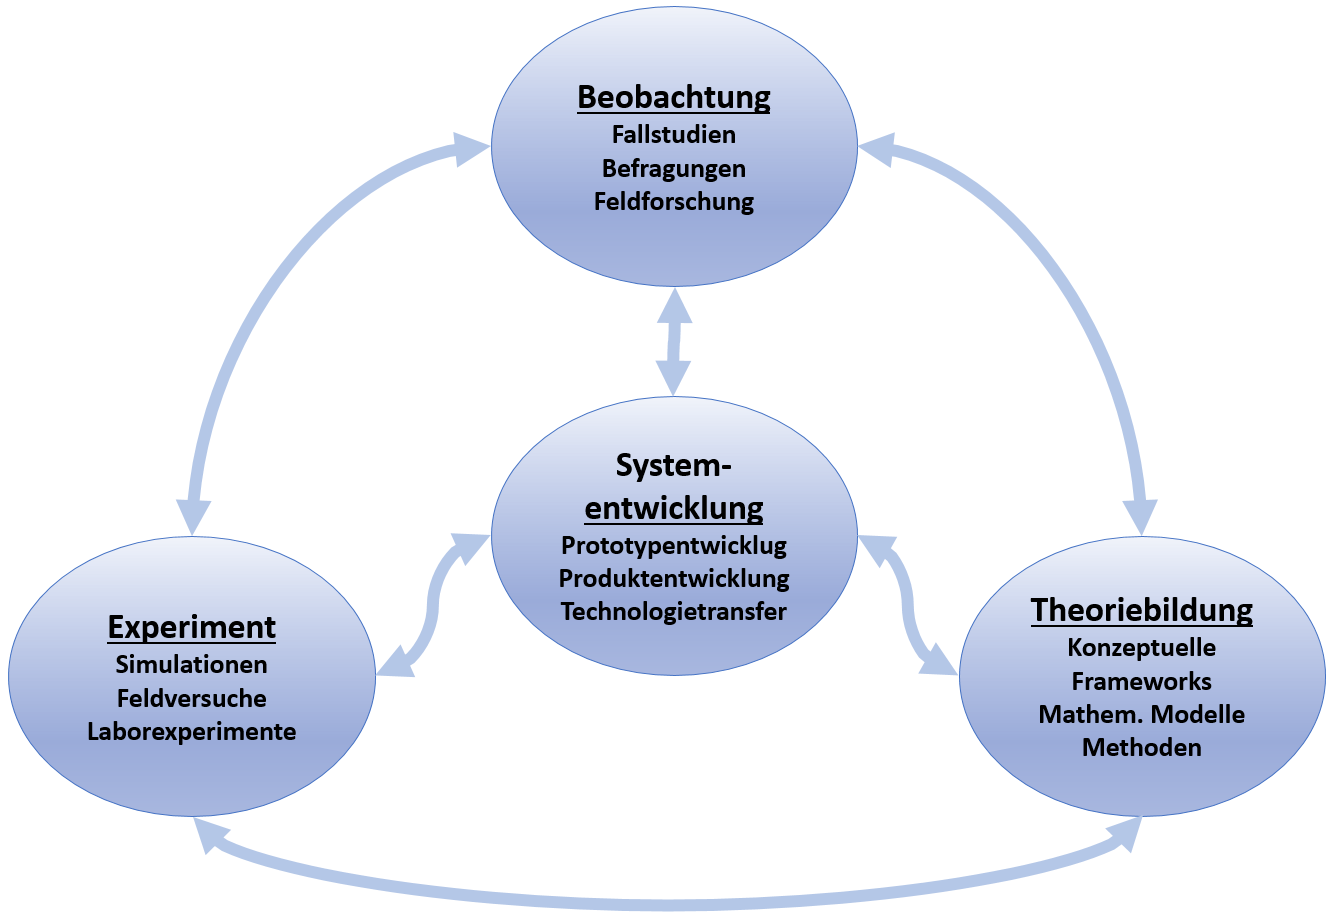
\includegraphics[width=\textwidth]{pictures/Nunamaker2.png}
    \caption{Forschungsmethode nach \cite{nunamaker_systems_1990-1}}
    \label{fig:nunamaker}
\end{figure}

Die Forschungsmethode umfasst die folgenden in Abbildung \ref{fig:nunamaker} dargestellten Phasen:
\begin{description}
\item[Beobachtung:] Insbesondere wenn der Untersuchungsgegenstand relativ unbekannt ist, werden Fallstudien, Feldversuche oder Umfragen durchgeführt, um ein \glqq Gefühl\grqq{} für den Aufwand zu erhalten. Auf dieser Grundlage können dann konkrete Hypothesen erstellt werden, die durch Experimente geprüft werden. 

In dieser Arbeit findet aufgrund der Art des Untersuchungsgegenstandes in der Beobachtungsphase hauptsächlich die Literaturrecherche und Ermittlung des Standes von Wissenschaft und Technik statt.

\item[Theoriebildung:] In dieser Phase werden neue Ideen, Konzepte Methoden oder Modelle entwickelt. Diese Theorien beschreiben das Systemverhalten allgemein, haben jedoch wenig praktische Bedeutung für die Zieldomäne. Sie können aber genutzt werden, um Forschungshypothesen aufzustellen, die Planung von Experimenten zu unterstützen und systematische Beobachtungen durchzuführen.

\item[Systementwicklung:] Diese Phase besteht aus fünf Teilen:
\begin{itemize}
\item Konzeptentwurf

\item Erstellung der Systemarchitektur

\item Erstellung von Prototypen

\item Produktentwicklung

\item Technologietransfer
\end{itemize}


\item[Experiment:] In dieser Phase werden die gefundenen Theorien und entwickelten Systeme evaluiert. Die Ergebnisse der Experimente können genutzt werden, um die Theorien weiterzuentwickeln und die Systeme zu verbessern.

\end{description}

Obwohl die Phasen in der Methode keine vorgegebene Reihenfolge haben, sondern sich gegenseitig beeinflussen, wird in der vorliegenden Arbeit die oben angeführte Abfolge verwendet.


% !TEX root =expose.tex
\chapter{Lösungsansatz}

Die Wissensrepräsentation medizinischer Texte soll Entitäten unterschiedlicher Kategorie miteinander in Beziehung setzen. Naheliegend ist es z.B., automatisch in einem Text Symptome und Krankheiten zu identifizieren, diese miteinander in Beziehung zu setzen und eine Wissensrepräsentation der Art

\begin{center}
loss of appetite - is a symptom of - depression
\end{center}

zu erzeugen. Dazu muss spaCy befähigt werden, nicht nur Fachbegriffe zu erkennen, sondern diese auch richtig zu kategorisieren, als z.B. Krankheit oder Symptom. Folgender Lösungsansatz ist angedacht:

MetaMapLite verwendet eine auf UMLS basierende Datenbasis mit medizinischen Fachbegriffen. Der Umfang der Datenbasis von MetaMapLite ist etwas reduziert und umfasst z.B. nur englische Fachbegriffe. Auf der MetaMapLite-Website kann das zip-Archiv

\begin{center}
\emph{public\_mm\_data\_lite\_usabase\_2022aa}
\end{center}

heruntergeladen werden. In diesem Archiv befindet sich die Datei \emph{postings} in dem Unterordner

\begin{center}
\emph{\textbackslash public\_mm\_lite\textbackslash data\textbackslash ivf \textbackslash 2022AA\textbackslash USAbase\textbackslash indices\textbackslash cuisourceinfo}.
\end{center}

Die Datei \emph{postings} enthält ca. 11 Millionen englischsprachige Einträge und ist mit einer Größe von etwa 739 MB etwas handlicher als die Datenbestände von UMLS. Um zu prüfen, ob diese Datenbasis geeignet ist, ist ein Auszug von Einträgen, die für den zu analysierenden Beispieltext über Depressionen relevant sind, in der folgenden Tabelle aufgelistet.

CUI bezeichnet den Concept Unique Identifier, mit dem Synonyme gefunden werden können. Der CUI besteht nur aus dem mit dem Buchstaben `C' beginnenden Teil und ist hier ergänzt durch einen sogenannten Term-Type. Der Term-Type `PT' kennzeichnet z.B. bevorzugte Einträge. SUI bezeichnet den String Unique Identifier, mit dem gleichlautende (und damit redundante) Bezeichnungen gefunden werden können.

Die Tabelle listet nur Einträge auf, in denen der Begriff, z.B. `depression', einer in Klammern hinter dem Begriff stehenden Kategorie zugeordnet ist, hier z.B. `disease'. Über den CUI können in der Datei \emph{postings} Synonyme gefunden werden, wobei nur der mit `C' beginnende Teil relevant ist. Diese Synonyme enthalten häufig keine Kategorien in Klammern. Die Kategorien können aber über den CUI den Synonymen zugeordnet werden. Die sehr zahlreichen Synonyme bzw. alternativen Ausdrücke sind in der Tabelle nicht aufgeführt.

\begin{center}
\begin{tabular}{llll}
\hline
\textbf{CUI}	& \textbf{SUI}	& \textbf{Item} & \textbf{Source} \\
\hline
FNC0232933 &	S3225525 & \parbox[t]{5cm}{Abnormal menstrual cycle (finding)} &	SNOMEDCT\_US \\
PTC0424569 &	S3221759 & \parbox[t]{5cm}{Circumstances interfere with sleep (disorder)} &	SNOMEDCT\_US \\
YC0009806 & S3235964 & Constipation (finding) &	SNOMEDCT\_US \\
LAC3845528 &	S14560529 &\parbox[t]{5cm}{Depressed mood (e.g., feeling sad, tearful)} & LNC \\
SYC0344315 &	S3252744 &	Depressed mood (finding) &	SNOMEDCT\_US \\
GTC0011570 &	S1431189 &	depression (disease) & AOD \\
SYC0681028 &	S1431190 &	depression (economic) & AOD \\
ETC0021603 &	S3263624 &	\parbox[t]{5cm}{Disorders of initiating and maintaining sleep (disorder)} & SNOMEDCT\_US \\
FNC2939186 &	S3264511 &	Disturbance in mood (finding) & SNOMEDCT\_US \\
SYC0349217 &	S20166983 & Episode of depression (finding) & SNOMEDCT\_US \\
FNC1288289 &	S3312713 &	Fearful mood (finding) & SNOMEDCT\_US \\
FNC0150041 &	S3313279 &	Feeling hopeless (finding) &	SNOMEDCT\_US \\
FNC0022107 &	S3313282 &	Feeling irritable (finding)	 & SNOMEDCT\_US \\
FNC0424000 &	S3313310 &	Feeling suicidal (finding) &	SNOMEDCT\_US \\
ETC0917801 &	S3373158 &	Insomnia (disorder) &	SNOMEDCT\_US \\
PTC0015672 &	S3386372 &	Lack of energy (finding) &	SNOMEDCT\_US \\
FNC2981158 &	S3386389 &	Lack of libido (finding) & SNOMEDCT\_US \\
FNC1971624 &	S3397609 &	Loss of appetite (finding) & SNOMEDCT\_US \\
FNC0178417 &	S3397620 &	\parbox[t]{5cm}{Loss of capacity for enjoyment (finding)} & SNOMEDCT\_US \\
FNC0456814 &	S3397668 &	Loss of motivation (finding)  & SNOMEDCT\_US \\
FNC0424219 &	S3397688 &	Loss of self-esteem (finding) & SNOMEDCT\_US \\
FNC0679136 &	S3398077 &	Low self-esteem (finding) & SNOMEDCT\_US \\
PTC5444612 &	S20749480 & mood (physical finding) & MTH \\
FNC0424566 &	S3439673 &	\parbox[t]{5cm}{Not getting enough sleep (disorder)} &	SNOMEDCT\_US \\
FNC2945580 &	S3485453 &	Poor self-esteem (finding) &	SNOMEDCT\_US \\
FNC0235160 &	S3513783 &	Restless sleep (finding) & SNOMEDCT\_US \\
FNC0424570 &	S3580589 &	\parbox[t]{5cm}{Symptoms interfere with sleep (disorder)} & SNOMEDCT\_US \\
PTC0424570 &	S3580589 &	\parbox[t]{5cm}{Symptoms interfere with sleep (disorder)} & SNOMEDCT\_US \\
PTC0233481 &	S3620195 &	Worried (finding) & SNOMEDCT\_US \\
\hline
\end{tabular}
\end{center}

In der Tabelle finden sich drei Kategorien, `disease', `disorder' und `finding' (Die \emph{postings}-Datei enthält noch viele andere). Hier bietet sich an, die Begriffe und Kategorien dieser Datenbasis für das Trainieren des EntityRecognizers von spaCy zu verwenden. Die Zuordnung `finding' ist hier stets als Symptom zu verstehen. `disorder', also Störung, kennzeichnet in den meisten Fällen ebenfalls eine Krankheit. Der Begriff `insomnia' findet sich nicht im zu analysierenden Text, dort ist stattdessen von `disturbed sleep' die Rede ist. Hier muss versucht werden, über Synonyme eine richtige Kategorisierung zu erreichen. Die meisten Einträge stammen von der Datenbank SNOMED CT (Systematized Nomenclature of Medicine Clinical Terms), die seit 2003 Teil des UMLS Metathesaurus ist. 

Der Inhalt der Datei \emph{postings} muss aufbereitet (und ggf. auch gekürzt) werden, so dass die Daten für das Training des EntityRecognizers verwendet werden können. Es muss untersucht werden, wie basierend auf der Wörterliste geeignete Trainingsdaten erzeugt werden können, etwa durch automatisch erzeugte Beispielsätze.

Der zu analysierende Text muss durch ein Python-Programm aufbereitet werden, mit dem Ziel, dass die NLP-Komponenten der Prozesspipeline des NLP-Frameworks, möglichst erfolgreich arbeiten. Ein Vorgehen könnte sein, Aufzählungen in mehrere vollständige Sätze zu zerlegen, so dass möglichst sinnvolle vollständige Sätze entstehen, die eine Krankheit und ein Symptom enthalten, so dass die automatische Textanalyse nicht überfordert wird, Krankheit und Symptome zusammenzubringen. Hierbei werden die von spaCy zur Verfügung gestellten Pipeline-Komponenten wie der Lemmatizer und Parser genutzt.

Idealerweise entsteht so ein Text mit Aussagesätzen, die jeweils eine Krankheit und ein oder mehrere Symptome enthalten. Für die Wissensrepräsentation soll der EntityLinker eingesetzt werden. Normalerweise wird der EntityLinker verwendet, um (mehrdeutige) Entitäten, die vom EntityRecognizer oder EntityRuler gefunden werden, einer eindeutigen Entität zuzuordnen (z.B. einem Wikipedia-Eintrag). Der EntityLinker wird trainiert, so dass die Zuordnung Kontext-basiert erfolgt.

Für die Erstellung der Wissensrepräsentation wird der EntityLinker auf unorthodoxe Weise verwendt und mit dieser Komponente die Wissensrepräsentation aufgebaut. Dafür ist die Wissensbasis des EntityLinkers von zentraler Bedeutung. In dieser werden durch das Python-Programm als zusammengehörend erkannte Krankheiten und Symptome gespeichert. Dabei können Symptome mehreren Krankheiten zugeordnet werden. Der EntityLinker wird mit Sätzen aus den zu analysierenden Texten trainiert, die es ihm erlauben, auch bei anderen Texten Kontext-basiert einem Symptom die richtige Krankheit zuzuordnen. Analysiert man viele Text hintereinander, kann der EntityLinker so mit der Zeit eine umfangreiche Wissensbasis aufbauen. Analysiert man einen Text dann mit dem Entity Recognizer und danach mit dem EntityLinker, dann entsteht automatisch die Wissensrepräsentation, wobei etwa die Entität `lack of energy' vom EntityRecognizer gefunden wird und als `Symptom' kategorisiert wird und anschließend vom EntityLinker der Krankheit `depression' zugeordnet wird, sofern sich dies auch dem Kontext ergibt.

\vspace{1cm}

Arbeitspakete:
\begin{itemize}
    \item Manuelle Erstellung einer Wissensrepräsentation basierend auf dem zu analysierenden Text
    \item Identifizierung eines medizinischen Vokabulars, das zum Training der NER-Komponente verwendet werden kann
    \item Untersuchung, auf welche Weise die Trainingsdaten für möglichst gute Ergebnisse der NER-Komponente aufbereitet werden müssen (z.B. durch automatisch erzeugte Beispielsätze)
    \item Entwicklung einer Programm-Komponente, die die zu analysierenden Texte vorverarbeitet, so dass die NLP-Pipeline möglichst effizient arbeitet
    \item Entwicklung ein Programm-Komponente, die basierend auf den vom NER gefundenen Entitäten zusammengehörende Entitäten (etwa Symptom und Krankheit) identifiziert und zusammen mit Beispielsätzen aus dem zu analysierenden Text die Wissensbasis des EntityLinkers aufbaut.
    \item Entwicklung der Programm-Komponente, die die Wissensbasis des EntityLinkers ausgewertet, und in eine XML-Datei o.ä. exportiert. Anschließend Darstellung als RDF-Modell.
\end{itemize}




\chapter{Stand der Wissenschaft}
\label{ch:standderwissenschaft} 


%
% Section: FZ 1.1. Aufbau und Struktur medizinischer Texte 
%
\section{FZ 1.1. Aufbau und Struktur medizinischer Texte}
\label{sec:fz1.1.} 

Medizinische Texte existieren in verschiedenen Formen mit unterschiedlichen Zielsetzungen. Beispielsweise gibt es Lehrbuch- und Enzyklopädietexte, die überblicksweise über medizinische Sachverhalte informieren, wissenschaftliche Studien, in denen neue wissenschaftliche Erkenntnisse vorgestellt werden und außerdem Arztberichte, in denen über individuelle Patienten und deren Krankheitsverlauf informiert wird.
Die für diese Arbeit genutzten Analysetexte stellen enzyklopädische Texte dar, in denen insbesondere Symptome und Merkmale psychologischer Erkrankungen beschrieben werden.
Charakterisiert sind diese Texte dadurch, dass sie durch Zwischenüberschriften gegliedert sind und neben Fließtext auch Aufzählungen enthalten.


%
% Section: FZ 2.1. Überblick über depressive Erkrankungen 
%
\section{FZ 2.1. Überblick über depressive Erkrankungen}
\label{sec:fz2.1.} 
Als Quellen für diesen Abschnitt dienten \cite{mpg_depression}, \cite{who_depression} und \cite{psychrembel_depression}.
\subsection{Allgemein}
Depression ist eine psychische Krankheit, die geschätzt $3,8 \%$ der Weltbevölkerung und $5\%$ der Erwachsenen betrifft.
Sie kann dazu führen, dass betroffene Menschen Schwierigkeiten haben im Arbeits- und Familienleben zurecht zu
kommen.

\subsection{Symptome}
Übliche Symptome eine Depression sind eine traurige Grundstimmung, Konzentrationsprobleme, Hoffnungslosigkeit, 
Müdigkeit und Reizbarkeit. Auch Schlafstörungen, eine Libidostörung, verminderter oder gesteigerter Appetit und
ein vermindertes Selbswertgefühl oder Selbstbewusstsein sind Symptome. Im schlimmsten Fall treten 
Selbsttötungsgedanken auf.

\subsection{Formen der Depression}
Die Schwere einer typischen Depression wird durch leichte, mittelgradige und schwere Episoden unterschieden. Dabei 
sind die Übergänge fließend.
Besondere Formen der Depression sind die chronische Depression, bei der trotz therapeutischer Maßnahmen nur wenig 
Besserung eintritt. Des Weiteren gibt es die manisch-depressive Depression, bei der sich depressive und manische 
Phasen abwechseln. Außerdem gibt es auch kurze, akute depressive Verstimmungen, die nur zwischen einem Tag und
zwei Wochen dauern. 

\subsection{Ursachen}
Depressionen entstehen durch ein komplexes Zusammenspiel von sozialen, psychologischen und biologischen Faktoren.
Dabei wird angenommen, dass für eine typische Depression die Genetik $50 \%$ der Ursachen ausmacht. 
Konkret können Kindheitserfahrungen, Verluste und Arbeitslosigkeit eine Depression begünstigen.

\subsection{Behandlung}
Je nach Schweregrad der Krankheit werden zur Behandlung von Depressionen psychologische Behandlungen angewandt, 
und/oder den betroffenen Personen Antidepressiva verschrieben.


%
% Section: FZ 2.2. Automatisierung durch NLP 
%
\section{FZ 2.2. Automatisierung durch NLP}
\label{sec:fz2.2.} 

\subsection{Natural Language Processing (NLP)}
Natural Language Processing ist ein Teil der Künstlichen Intelligenz. Er befasst sich mit der Aufgabe
Maschinen den Umgang mit der menschlichen Sprache beizubringen, also das Verstehen der Sprache und dem
richtigen Antworten darauf. Mithilfe von NLP-Methoden werden zum Beispiel Sätze analysiert, die Bedeutung 
von Texten erfasst, Chatbots erstellt und sogar ganze Geschichten geschrieben.
Die grundlegendsten Schritte, die beim Erarbeiten eines NLP-Modells (oder allgemeiner eines 
Machine-Learning-Modells) ausgeführt werden, sind folgende:
\begin{enumerate}
	\item Aufbereitung von Daten
	\item Wählen eines geeigneten Algorithmus
	\item Trainieren des Modells mit Trainingsdaten
	\item Testen des Modells mit Testdaten
	\item Modell anwenden / Vorhersagen treffen
\end{enumerate}

\subsection{Named Entity Recognition (NER)}
Named Entity Recognition bezeichnet einen Teilbereich des Natural Language Processing, bei dem es darum geht 
wichtige Entitäten, wie zum Beispiel Personen, Orte oder Institutionen, in einem Text zu erkennen. Methoden 
zur Bewältigung dieser Aufgabe werden seit circa 30 Jahren entwickelt. Darunter fallen grammatikbasierte und 
statistische Methoden, sowie auch Methoden des Machine Learning.

\subsection{Entity Linking}
Als Entity Linking wird im Bereich des NLP die Aufgabe beschrieben, die den Entitäten (z.B. Personen, Orte) 
in einem Text das korrekte Äquivalent in einer Wissensbasis zuordnen soll.
In \cite{shen_entity_2021} wird Entity Linking folgendermaßen definiert (übersetzt):
\begin{defn}[Entity Linking]
Gegeben sei ein Dokument $D$, welches die erkannten Entitäten $M=\{m_1, m_2, \dots, m_{|M|}\}$ enthält, sowie
eine Ziel-Wissensbasis $KB$, welches die Entitäten $E=\{e_1, e_2, \dots, e_{|M|}\}$ enthält. Das Ziel ist es 
jede Entität $m_i$ in $M$ seinem korrekten Äquivalent $e_i$ in $E$ zuzuordnen.
\end{defn}

\subsection{spaCy}
spaCy ist eine Python-Bibliothek, die die erforderlichen Daten und Algorithmen enthält, die zum verarbeiten von
Texten mit natürlicher Sprache benötigt werden. SpaCy enthält vortrainierte Modelle für über 70 verschiedene 
Sprachen, unter anderem Spanisch, Englisch, Griechisch und Deutsch. Zudem ermöglicht spaCy das Einbinden von 
Modellen, die mithilfe anderer Python-Bibliotheken (zum Beispiel PyTorch oder TensorFlow) trainiert wurden.
Anders als einige andere NLP-Bibliotheken konzentriert sich spaCy darauf, Software für den Produktionseinsatz 
zur Verfügung zu stellen. Erstmals wurde spaCy 2015 von Matthew Honnibal veröffentlicht. 
(\cite{vasiliev2020natural}, \cite{github_spacy}, \cite{spacy})

\subsection{Weitere Python-Bibliotheken für Machine Learning (ML) und NER}
Eine der wichtigsten Python-Bibliotheken für NLP ist NLTK (Natural Language Toolkit) (\cite{bird2006nltk}).
Weitere Python-Bibliotheken, die für NLP-Aufgaben genutzt werden können, sind unter Anderem
Gensim (\cite{vrehuuvrek2011gensim}), Pattern (\cite{de2012pattern}, \cite{github_pattern}), 
scikit-learn und PyTorch.

%
% Section: FZ 1.1. Wissensrepräsentation mittels RDF
%
\section{FZ 3.1. Wissensrepräsentation mittels RDF}
\label{sec:fz3.1.} 

Das \emph{Resource Description Framework} (RDF) \cite{w3c_all_2022} ist ein Framework zur Darstellung von Informationen im Semantischen Web, das von der \emph{RDF Working Group} des  \emph{World Wide Web Consortium} (W3C) erstellt wurde. Das RDF-Modell besteht aus einem Datenmodell, mit dem Aussagen über Ressourcen in Form eines Graphen dargestellt werden. Die Informationen werden als Tripel von Subjekt, Prädikat und Objekt gespeichert und ermöglichen auf diese Weise eine maschinenlesbare Bereitstellung semantischer Informationen.

Die Subjekte und Objekte sind dabei die Knoten des Graphen und die Prädikate die Kanten zwischen diesen Knoten.

Abbildung \ref{fig:rdfgraph} zeigt einen einfachen RDF-Graphen, in dem das Subjekt \glqq depression\grqq{} mit dem Prädikat \glqq hasSymptom\grqq{} mit zwei Symptomen verbunden und über das Prädikat \glqq isA\grqq{} mit dem Objekt \glqq mentalDisorder\grqq{} verbunden ist.

\begin{figure}[h]
    \centering
    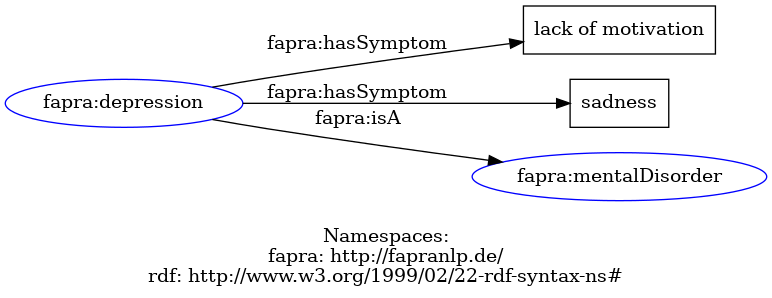
\includegraphics[width=\textwidth]{pictures/rdf-graph.png}
    \caption{einfacher RDF-Graph (visualisiert mit \url{https://www.ldf.fi/service/rdf-grapher}}
    \label{fig:rdfgraph}
\end{figure}

\subsection{Resource Description Framework Schema}

Zusätzlich zu RDF stellt das W3C auch eine Empfehlung für ein Datenmodellierungsvokabular für RDF-Daten bereit: das RDF-Schema. Dies stellt eine Erweiterung des grundlegenden RDF-Vokabulars dar. \dots{} [TODO]

\subsection{Dublin Core Metadata Initiative}
DCMI \dots{} [TODO]

\subsection{Serialisierung von RDF-Graphen}

Für die Serialisierung von RDF-Graphen stehen mehrere Formate zur Verfügung. So wird der MeSH-Datensatz im \emph{N-Triples}-Format bereitgestellt und in diesem Praktikum erfolgt die Ausgabe der Wissensrepräsentation im RDF/XML-Format.

Ein Beispiel für die Serialisierung des in Abbildung \ref{fig:rdfgraph} dargestellten Graphen im RDF/XML-Format ist in Listing \ref{listing:rdfxml} angeführt.

\lstset{language=XML, caption=RDF/XML, label=listing:rdfxml}
\begin{lstlisting}
<?xml version="1.0" encoding="utf-8"?>
<rdf:RDF
  xmlns:fapra="http://fapranlp.de/"
  xmlns:rdf="http://www.w3.org/1999/02/22-rdf-syntax-ns#"
>
  <rdf:Description rdf:about="http://fapranlp.de/depression">
    <fapra:hasSymptom>lack of motivation</fapra:hasSymptom>
    <fapra:hasSymptom>sadness</fapra:hasSymptom>
    <fapra:isA rdf:resource="http://fapranlp.de/mentalDisorder"/>
  </rdf:Description>
</rdf:RDF>
\end{lstlisting}




Für Python steht mit RDFLib \cite{rdflib_team_rdflib_2022} eine Bibliothek zur Arbeit mit RDF-Graphen bereit.

\subsection{SPARQL Protocol and RDF Query Language}
SPARQL \dots{} [TODO]
% !TEX root =expose.tex
\chapter{Arbeits- und Zeitplan}

\begin{figure}[h]
    \centering
    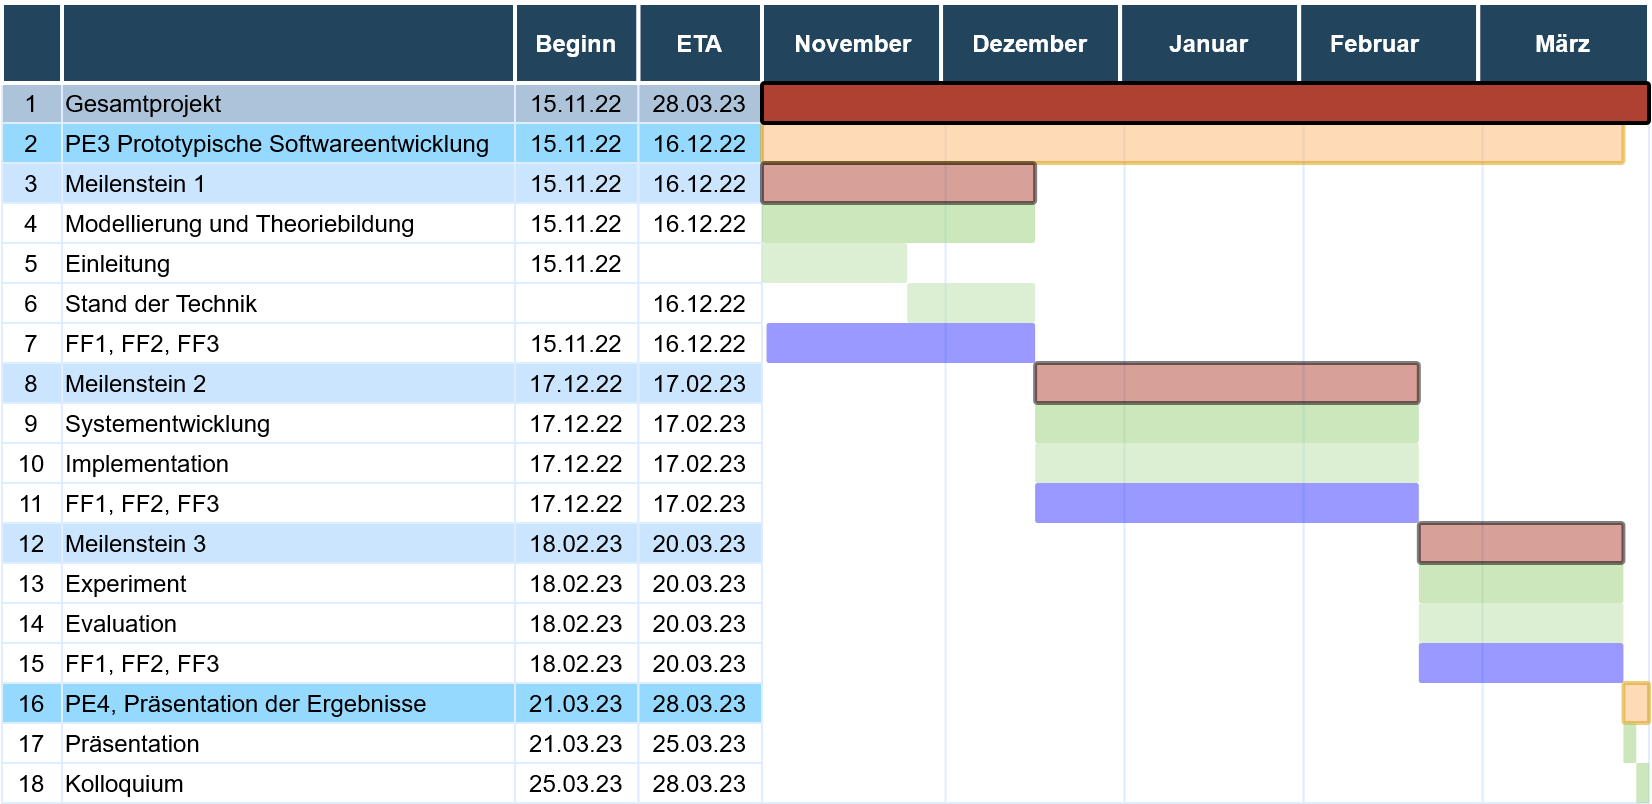
\includegraphics[width=\textwidth]{pictures/zeitplan.png}
    \caption{Arbeits- und Zeitplan}
    \label{fig:zeitplan}
\end{figure}

 

\bibliographystyle{abbrv}
%\usepackage[style=ieee-alphabetic, backend=biber, natbib=true]{biblatex}
%\addbibresource{literatur.bib}
%\bibliography{literatur} % Daten aus der Datei literatur.bib verwenden.
\end{document}
